% Syllabus Template from Arman Shokrollahi
% https://www.overleaf.com/latex/templates/syllabus-template-course-info/gbqbpcdgvxjs

\documentclass[11pt, letterpaper]{article}
%\usepackage{geometry}
\usepackage[inner=2cm,outer=2cm,top=2.5cm,bottom=2.5cm]{geometry}
\pagestyle{empty}
\usepackage{graphicx}
\usepackage{fancyhdr, lastpage, bbding, pmboxdraw}
\usepackage[usenames,dvipsnames]{color}
\definecolor{darkblue}{rgb}{0,0,.6}
\definecolor{darkred}{rgb}{.7,0,0}
\definecolor{darkgreen}{rgb}{0,.6,0}
\definecolor{red}{rgb}{.98,0,0}
\usepackage[colorlinks,pagebackref,pdfusetitle,urlcolor=darkblue,citecolor=darkblue,linkcolor=darkred,bookmarksnumbered,plainpages=false]{hyperref}
\renewcommand{\thefootnote}{\fnsymbol{footnote}}

\pagestyle{fancyplain}
\fancyhf{}
\lhead{ \fancyplain{}{Introduction to Political Methodology} }
%\chead{ \fancyplain{}{} }
\rhead{ \fancyplain{}{Fall 2023} }%\today
%\rfoot{\fancyplain{}{page \thepage\ of \pageref{LastPage}}}
\fancyfoot[RO, LE] {page \thepage\ of \pageref{LastPage} }
\thispagestyle{plain}

%%%%%%%%%%%% LISTING %%%
\usepackage{listings}
\usepackage{caption}
\DeclareCaptionFont{white}{\color{white}}
\DeclareCaptionFormat{listing}{\colorbox{gray}{\parbox{\textwidth}{#1#2#3}}}
\captionsetup[lstlisting]{format=listing,labelfont=white,textfont=white}
\usepackage{verbatim} % used to display code
\usepackage{fancyvrb}
\usepackage{acronym}
\usepackage{amsthm}
\VerbatimFootnotes % Required, otherwise verbatim does not work in footnotes!



\definecolor{OliveGreen}{cmyk}{0.64,0,0.95,0.40}
\definecolor{CadetBlue}{cmyk}{0.62,0.57,0.23,0}
\definecolor{lightlightgray}{gray}{0.93}



\lstset{
%language=bash,                          % Code langugage
basicstyle=\ttfamily,                   % Code font, Examples: \footnotesize, \ttfamily
keywordstyle=\color{OliveGreen},        % Keywords font ('*' = uppercase)
commentstyle=\color{gray},              % Comments font
numbers=left,                           % Line nums position
numberstyle=\tiny,                      % Line-numbers fonts
stepnumber=1,                           % Step between two line-numbers
numbersep=5pt,                          % How far are line-numbers from code
backgroundcolor=\color{lightlightgray}, % Choose background color
frame=none,                             % A frame around the code
tabsize=2,                              % Default tab size
captionpos=t,                           % Caption-position = bottom
breaklines=true,                        % Automatic line breaking?
breakatwhitespace=false,                % Automatic breaks only at whitespace?
showspaces=false,                       % Dont make spaces visible
showtabs=false,                         % Dont make tabls visible
columns=flexible,                       % Column format
morekeywords={__global__, __device__},  % CUDA specific keywords
}

%%%%%%%%%%%%%%%%%%%%%%%%%%%%%%%%%%%%
\begin{document}
\begin{center}
{\Large \textsc{POLS 7012: Introduction to Political Methodology}}
\end{center}
\begin{center}
{\large Fall 2023}
\end{center}

\begin{center}
\rule{6.5in}{0.4pt}
\begin{minipage}[t]{.96\textwidth}
\begin{tabular}{llcccll}
\textbf{Professor:} & Joe Ornstein & & &  & \textbf{Time:} & W 3:55 -- 6:40pm \\
\textbf{Email:} &  \href{mailto:jornstein@uga.edu}{jornstein@uga.edu} & & & & \textbf{Place:} & 302 Baldwin Hall\\
\textbf{Website:} & \href{https://joeornstein.github.io/pols-7012/}{https://joeornstein.github.io/pols-7012/} & & & & &
\end{tabular}
\end{minipage}
\rule{6.5in}{0.4pt}
\end{center}
\vspace{.15cm}
\setlength{\unitlength}{1in}
\renewcommand{\arraystretch}{2}


\noindent So you want to be a political scientist? Cool! It's a fun and fulfilling profession. But before you can eat your cake, you need to eat your vegetables. In this analogy, cake is political science, and vegetables is math. Because modern political science is heavily quantitative, and in order to fruitfully engage with the ongoing scientific conversation, you will need to understand the language.

I intend for this class to be a very practical introduction to the mathematical and computational skills you'll want to have as a professional political scientist. In Part 1 of the course (Discovery), you'll learn the programming skills you need to tidy, explore, and describe patterns in data. In Part 2 (Causality), you'll learn how to design research that convincingly distinguishes between correlation and causation. In Part 3 (Uncertainty), you'll learn the foundational statistical tools you need to communicate the uncertainty of your estimates and to generalize from samples to populations. And when we're done, you'll have the fundamentals you need to tackle the advanced material that makes up the rest of the methods sequence.

\begin{figure}[h]
	\centering
	\href{https://xkcd.com/1856/}{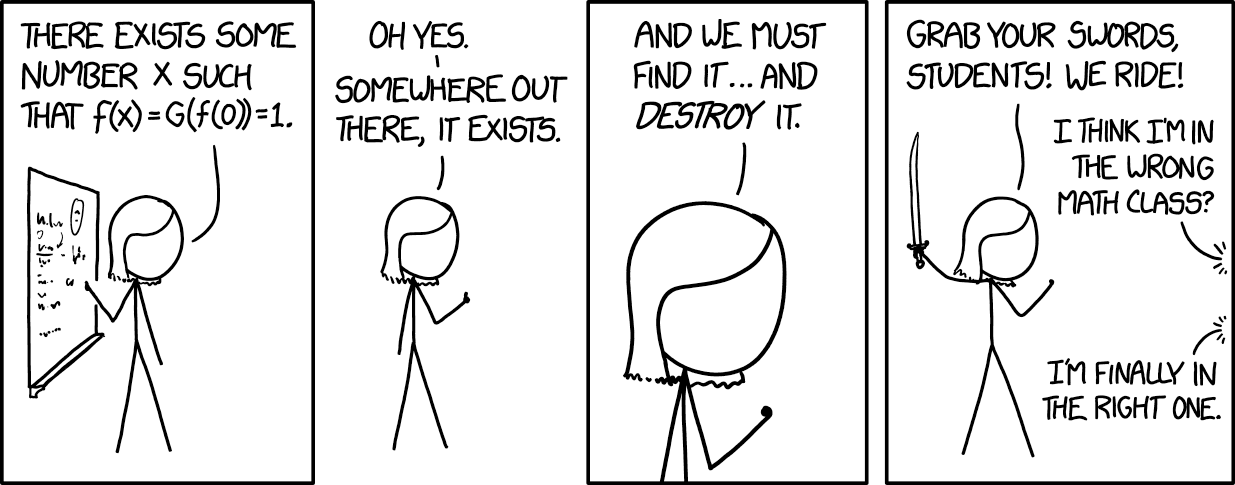
\includegraphics[width=0.8\textwidth]{img/existence_proof_2x.png}}
\end{figure}

%\begin{quotation}
%	\noindent``\textit{You can't really know anything if you just remember isolated facts. If the facts don't hang together on a latticework of theory, you don't have them in a usable form. You've got to have models in your head.}''\\
%	\\
%	--Charlie Munger (investor, vice chairman of Berkshire Hathaway)
%\end{quotation}


\section*{Course Objectives}
%\vskip.15in
%\noindent\textbf{Course Objectives:}
By the end of this course, you will be able to:
\begin{itemize}
	\item Confidently work with data using the \texttt{R} programming language
	\item Create beautiful and informative data visualizations
	\item Organize your work so that it is transparent and reproducible
	\item Build basic statistical models and estimate their parameters from data
	\item Communicate the uncertainty around your estimates
	\item Describe research designs that can credibly identify causation (not just correlation)
%	\item Explain the fundamental mathematics behind the statistical methods we use in political science (probability and inference, matrix algebra, and optimization).
%	\item Manipulate, wrangle, and clean datasets using the \texttt{R} programming language
%	\item Create beautiful data visualizations
%	\item Organize your work so that it is transparent and reproducible
%	\item Compute derivatives and solve systems of linear equations
%	\item Explain the properties of probability distributions and expected values
%	\item Perform hypothesis tests and fit models to data
\end{itemize}

%\section*{Course Structure}
%
%This will be a weird semester, and I expect that there will be more than the usual share of setbacks and hardships. Please don't hesitate to ask questions or reach out to me with your concerns.
%
%If you show any \href{https://www.google.com/search?q=covid-19+symptoms}{symptoms of COVID-19} or have been exposed to someone who tests positive for COVID-19, don't come to class. Obviously. I do not grade class attendance, and every piece of material that you need to succeed on assignments and tests will be made available online. I plan to simulcast our class sessions over Zoom and post recordings to the course website, and I will hold regular virtual office hours if you have questions that aren't covered in those places.
%
%When you come to class, please wear a mask. The University System of Georgia (USG) requires all faculty, students, and staff to wear appropriate face coverings while inside campus buildings. Reasonable accommodations may be made for those who are unable to wear a face covering for documented health reasons. Students seeking an accommodation related to face coverings should contact Disability Services at \href{https://drc.uga.edu/}{https://drc.uga.edu/}. For more information on the University of Georgia's coronavirus response, visit \href{https://coronavirus.uga.edu/}{https://coronavirus.uga.edu/}.
%
%Our classroom will have a limited capacity this semester (14 students), but that should be sufficient to have all enrolled students attend in person. Following the Thanksgiving break, all remaining class sessions will be held online.

\section*{Assignments \& Grading}

Each week I will assign a problem set, due the Tuesday before class. Your responses will be graded for completion and reviewed in class. Feel free to work with your classmates, but please submit your answers individually. 70\% of your grade will come from these problem sets, and 15\% each from a midterm and final exam.

%\vskip.15in
%\noindent\textbf{Office Hours:}
\section*{Office Hours and Email Policy}
I will be available for meetings every Monday, Wednesday, and Friday afternoons, and you can sign up for 20 minute appointments \href{https://calendly.com/joeornstein/20min}{here}. My office is Baldwin 304C, but if you prefer we can talk over Zoom. If you send me an email, please allow me 24 hours to respond. Like many professors, my inbox is pretty overloaded. Also, I have small children, so it's my policy to not check email after 5pm or on weekends.

You should also feel free to seek assistance from the senior graduate students staffing the SPIA Methods Helpdesk. You can email them questions at \href{mailto:spia-methods-help@uga.edu}{spia-methods-help@uga.edu}.


%\vskip.15in
%\noindent\textbf{Textbook:} %\footnotemark
\section*{Books}
%All of the assigned readings for this class will be available free online (including a few of the textbooks listed below). However, if you're the sort of person that prefers reading hard copies, I recommend these books!

\begin{itemize}

%\item \href{https://www.amazon.com/Quantitative-Social-Science-Introduction-tidyverse/dp/0691222274}{Imai, Kosuke, and Nora Webb Williams (2022). \textit{Quantitative Social Science: An Introduction in Tidyverse}. Princeton: Princeton University Press.}

\item \href{https://press.princeton.edu/books/paperback/9780691199436/data-analysis-for-social-science}{Llaudet, Elena & Imai, Kosuke (2022). \textit{Data Analysis for Social Science: A Friendly and Practical Introduction}. Princeton University Press.}

\item \href{https://r4ds.hadley.nz/}{Wickham, H., Cetinkaya-Rundel, M., & Grolemund, G., (2023). \textit{R For Data Science: Import, Tidy, Transform, Visualize, and Model Data, 2nd Edition}. O'Reilly Media, Inc.}

\item \href{https://ebookcentral.proquest.com/lib/ugalib/detail.action?pq-origsite=primo&docID=1205618}{Moore, Will H., and David A. Siegel. 2013. \textit{A Mathematics Course for Political and Social Research}. Princeton, NJ: Princeton University Pres.}

\item \href{https://ebookcentral.proquest.com/lib/ugalib/reader.action?docID=3304559}{Strogatz, Steven H. 2012. \textit{The Joy of X: A Guided Tour of Math, from One to Infinity}. Boston: Houghton Mifflin Harcourt.}

%\item \href{https://theeffectbook.net/index.html.}{Huntington-Klein, Nick. 2021. \textit{The Effect: An Introduction to Research Design and Causality}. Chapman \& Hall CRC.}

%\item \href{https://www.amazon.com/Visual-Display-Quantitative-Information/dp/1930824130}{Tufte, Edward (2001). \textit{The Visual Display of Quantitative Information}}
%\item \href{https://socviz.co/}{Healy, Kieran (2018). \textit{Data Visualization: A Practical Introduction}. Princeton University Press.}




%\item \href{https://www.amazon.com/All-Statistics-Statistical-Inference-Springer/dp/1441923225}{Wasserman, L. (2013). \textit{All of Statistics: A Concise Course in Statistical Inference}. Springer Science \& Business Media.}
%\item \href{https://www.amazon.com/Mathematics-Economists-Carl-P-Simon/dp/0393957330}{Simon, C. P., \& Blume, L. (1994). \textit{Mathematics for Economists}. New York: Norton.}


\end{itemize}



\section*{Tentative Course Outline}

Moltke the Elder writes that no battle plan survives first contact with the enemy. This is doubly true for syllabi. We may need to be flexible, and deviate from the plan if some topics require more or less attention, or we think of something completely unexpected that we want to do, and it takes up a few weeks. Caveats aside, here is what I have planned! %I've built in some Bonus Weeks towards the end of the semester that we can use for catch up. If everything goes according to plan, then we can cover extra topics during those weeks by popular demand.

%\subsection*{PART 1: DISCOVERY}

%\begin{center}
%\begin{minipage}{6in}
%\begin{flushleft}
%Chapter 1 \dotfill ~$\approx$ 3 days \\
%{\color{darkgreen}{\Rectangle}} ~A little of probability theory and graph theory
\subsubsection*{Week 1: Getting Started}
\textit{Pre-Class Survey, Overcoming Fear, Setting Up R and RStudio}
\textbf{Reading}: None

\subsubsection*{Week 2: Writing Code}
\textit{Tidy Datasets, Variables, Basic Programming}
\textbf{Reading}: DAFSS Chapter 1

\subsubsection*{Week 3: Experiments}
\textit{The Fundamental Problem of Causal Inference, Potential Outcomes, Randomization, Estimation}
\textbf{Reading}: DAFSS Chapter 2

\subsubsection*{Week 4: Measurement}
\textit{Descriptive Statistics, Samples vs. Populations, Distributions}
\textbf{Reading}: DAFSS Chapter 3

\subsubsection*{Week 5: Visualization}
\textit{ggplot2, Distributions, Correlations, Conditional Distributions}
\textbf{Reading}: R4DS Chapter 1

\subsubsection*{Week 6: Tidying Data}
\textit{Importing, Merging, Data Wrangling}
\textbf{Reading}: R4DS Chapter 3 and 19

\subsubsection*{Week 7: Midterm Miniconference}

\subsubsection*{Week 8: Prediction}
\textit{The Linear Model, Logarithms}
\textbf{Reading}: DAFSS Chapter 4

\subsubsection*{Week 9: Calculus}
\textit{Derivatives, Optimization}
\textbf{Reading}: Moore & Siegel Chapter 5, Strogatz Chapter 17

%\subsubsection*{Week 3: Tools for Reproducible Research}
%\textit{Workflow, Documentation, File Structure, RMarkdown, \LaTeX, Zotero/Mendeley, \texttt{git} and GitHub}

%\subsubsection*{Week 5: Functions}
%\textit{Summation, Products, Logarithms, Exponentials, Writing Better Code, Flow Control}

%\subsubsection*{Week 7: Midterm}
%\textit{Mini-conference}

%\subsection*{PART 2: CAUSALITY}

\subsubsection*{Week 10: Causality}
\textit{Confounders, Multiple Regression, Internal and External Validity}
\textbf{Reading}: DAFSS Chapter 5

\subsubsection*{Week 11: Matrix Algebra}
\textit{Vectors, Matrices, Matrix Inverse, Ordinary Least Squares}
\textbf{Reading}: Moore & Siegel Chapter 12 (ignore sections 12.3.6 and 12.3.7).

%\subsubsection*{Week 10: Sneaking Through the Front Door}
%\textit{Experiments, Instrumental Variables, Regression Discontinuity}

%\subsection*{PART 3: UNCERTAINTY}

\subsubsection*{Week 12: Probability}
\textit{Sampling, Expected Value, Variance, Normal Distributions, Bernoulli Distributions, Central Limit Theorem, the Law of Large Numbers}
\textbf{Reading}: DAFSS Chapter 6

\subsubsection*{Weeks 13-14: Uncertainty}
\textit{Sampling Distributions, Standard Errors, Hypothesis Testing, p-values, Confidence Intervals, Integrals, The Fundamental Theorem of Calculus}
\textbf{Reading}: DAFSS Chapter 7


%\subsubsection*{Week 10: Matrix Algebra and OLS}
%\textit{Regression, Systems of Linear Equations, Independence, Matrix Multiplication, Matrix Inversion}
%
%\subsubsection*{Week 11: Models and Prediction}
%\textit{Fitting Models, Machine Learning, Overfitting, Cross-Validation, Regularization, Ensembles}

%\subsubsection*{Week 12: Bonus Week 1}
%Possible Topics: \textit{Causal Inference, Text-As-Data, Big Data, Machine Learning, Networks, Spatial Data, \texttt{blogdown, bookdown}, Advanced Reproducible Research}
%
%\subsubsection*{Week 13: Bonus Week 2}
%Possible Topics: \textit{Causal Inference, Text-As-Data, Big Data, Machine Learning, Networks, Spatial Data, \texttt{blogdown, bookdown}, Advanced Reproducible Research}
%
%\subsubsection*{Week 14: Bonus Week 3}
%Possible Topics: \textit{Causal Inference, Text-As-Data, Big Data, Machine Learning, Networks, Spatial Data, \texttt{blogdown, bookdown}, Advanced Reproducible Research}

\subsubsection*{Week 15: Wrap-Up}
\textit{Review, Catchup, Bonus Topics, Final Exam}



%\end{flushleft}
%\end{minipage}
%\end{center}

%\vskip.15in
%\noindent\textbf{Important Dates:}
%\begin{center} \begin{minipage}{3.8in}
%\begin{flushleft}
%Midterm \#1      \dotfill ~\={A}b\={a}n 16, 1393  \\
%Midterm \#2      \dotfill ~\={A}zar 21, 1393  \\
%%Project Deadline \dotfill ~Month Day \\
%Final Exam       \dotfill ~Dey 18, 1393  \\
%\end{flushleft}
%\end{minipage}
%\end{center}



\section*{Academic Honesty}
Remember that when you joined the University of Georgia community, you agreed to abide by a code of conduct outlined in the academic honesty policy called \href{https://honesty.uga.edu/Academic-Honesty-Policy/Introduction/}{\textit{A Culture of Honesty}}. Problem sets may be completed in groups, but I expect your responses to be individual, and the midterm and final must be completed individually.

\section*{Mental Health and Wellness Resources}

\begin{itemize}
\item If you or someone you know needs assistance, you are encouraged to contact Student Care and Outreach in the Division of Student Affairs at 706-542-7774 or visit \href{https://sco.uga.edu}{https://sco.uga.edu}. They will help you navigate any difficult circumstances you may be facing by connecting you with the appropriate resources or services.
\item UGA has several resources for a student seeking \href{https://www.uhs.uga.edu/bewelluga/bewelluga}{mental health services} or \href{https://www.uhs.uga.edu/info/emergencies}{crisis support}.
\item If you need help managing stress anxiety, relationships, etc., please visit \href{https://www.uhs.uga.edu/bewelluga/bewelluga}{BeWellUGA} for a list of FREE workshops, classes, mentoring, and health coaching led by licensed clinicians and health educators in the University Health Center.
\item Additional resources can be accessed through the UGA App.
\end{itemize}



%%%%%% THE END
\end{document}